%\documentclass[12pt]{article}
%\documentclass[12pt,dvips]{report}
\documentclass[12pt]{report}

\listfiles
%\usepackage{comment}
\usepackage{authblk} %for including author(s)


\usepackage[margin=2cm]{geometry} %for adjusting margins
\usepackage{pdfpages} %for including external PDFs

%for displaying source code, e.g., C++ code -------------------------------------
\usepackage{listings}
\usepackage{color}

\definecolor{mygreen}{rgb}{0,0.6,0}
\definecolor{mygray}{rgb}{0.5,0.5,0.5}
\definecolor{mymauve}{rgb}{0.58,0,0.82}

\lstset{ %
  backgroundcolor=\color{white},   % choose the background color; you must add \usepackage{color} or \usepackage{xcolor}
  basicstyle=\footnotesize,        % the size of the fonts that are used for the code
  breakatwhitespace=false,         % sets if automatic breaks should only happen at whitespace
  breaklines=true,                 % sets automatic line breaking
  captionpos=b,                    % sets the caption-position to bottom
  commentstyle=\color{mygreen},    % comment style
  deletekeywords={...},            % if you want to delete keywords from the given language
  escapeinside={\%*}{*)},          % if you want to add LaTeX within your code
  extendedchars=true,              % lets you use non-ASCII characters; for 8-bits encodings only, does not work with UTF-8
  frame=single,	                   % adds a frame around the code
  keepspaces=true,                 % keeps spaces in text, useful for keeping indentation of code (possibly needs columns=flexible)
  keywordstyle=\color{blue},       % keyword style
  language=Octave,                 % the language of the code
  otherkeywords={*,...},            % if you want to add more keywords to the set
  numbers=left,                    % where to put the line-numbers; possible values are (none, left, right)
  numbersep=5pt,                   % how far the line-numbers are from the code
  numberstyle=\tiny\color{mygray}, % the style that is used for the line-numbers
  rulecolor=\color{black},         % if not set, the frame-color may be changed on line-breaks within not-black text (e.g. comments (green here))
  showspaces=false,                % show spaces everywhere adding particular underscores; it overrides 'showstringspaces'
  showstringspaces=false,          % underline spaces within strings only
  showtabs=false,                  % show tabs within strings adding particular underscores
  stepnumber=2,                    % the step between two line-numbers. If it's 1, each line will be numbered
  stringstyle=\color{mymauve},     % string literal style
  tabsize=2,	                   % sets default tabsize to 2 spaces
  title=\lstname                   % show the filename of files included with \lstinputlisting; also try caption instead of title
}
%----------------------------------------------------------------------------------------------

%For table of contents ------------------------
\usepackage{graphicx}
\usepackage{epsf}
%\usepackage{hyperref}
\usepackage[breaklinks]{hyperref}
\usepackage{breakurl}
\usepackage{booktabs}

\usepackage{setspace}
\usepackage{amsmath}
\usepackage{algorithm}
\usepackage{algorithmic}
\usepackage{amsthm}
\usepackage{pdfpages}
\usepackage{bibentry}
%\usepackage{biblatex}
\nobibliography*

\usepackage{tocbibind} %add bib to TOC


%TODO command --------------------
\usepackage{color}
\definecolor{Orange}{rgb}{1,0.5,0}
\newcommand{\todo}[1]{\textsf{\textbf{\textcolor{Orange}{[[#1]]}}}}
%-------------------------------------------

\hypersetup{
    bookmarks=true,         	% show bookmarks bar?
    unicode=false,          	% non-Latin characters in Acrobat�s bookmarks
    pdftoolbar=true,        	% show Acrobat�s toolbar?
    pdfmenubar=true,        	% show Acrobat�s menu?
    pdffitwindow=false,     	% window fit to page when opened
    pdfstartview={FitH},    	% fits the width of the page to the window
    pdftitle={Chreston Allen Miller's PhD Dissertation},    	% title
    pdfauthor={Chreston Allen Miller},     % author
    pdfsubject={Behavior-Analysis},   % subject of the document
    pdfcreator={Chreston Allen Miller},   % creator of the document
    colorlinks=true,       % false: boxed links; true: colored links
    linkcolor=red,          % color of internal links
    linktoc=all,
    citecolor=red,        % color of links to bibliography
    filecolor=magenta,      % color of file links
    urlcolor=cyan           % color of external links
}
%----------------------------------------------------


\title{Software Documentation for Virginia Tech Smart Infrastructure Lab's DAQ Collection System}

%[1] for one author
\author[1]{ 
	Chreston Miller
}
\affil[1]{Research and Informatics, University Libraries, Virginia Tech}

\begin{document}% \sloppy
\maketitle

\tableofcontents

\pagebreak

\listoffigures

\chapter{Overview}
\label{ch:overview}
%\section{Overview}
This is documentation for the Collection System for the Virginia Tech Smart Infrastructure Lab's (VT SIL) building health monitoring system for Goodwin Hall at Virginia Tech. 

\section{Overview of System Design}
\label{sec:overview_of_system_design}

In Figure \ref{fig:daq_collection_system_design} in a high level outline of the system design and flow of operation. 
First, a connection is made with the specified DAQ(s). 
Then, the configuration parameters are loaded and the collection phase is initiated given the parameters. 
After a specified amount of time (from the configuration parameters) the data is written to a file. 
After which the collection cycle begins again. 
The collection system can be shutdown anytime. 
When shutdown, any currently held data is written to file and the connection to the DAQ(s) is closed. 

\begin{figure}
\centering
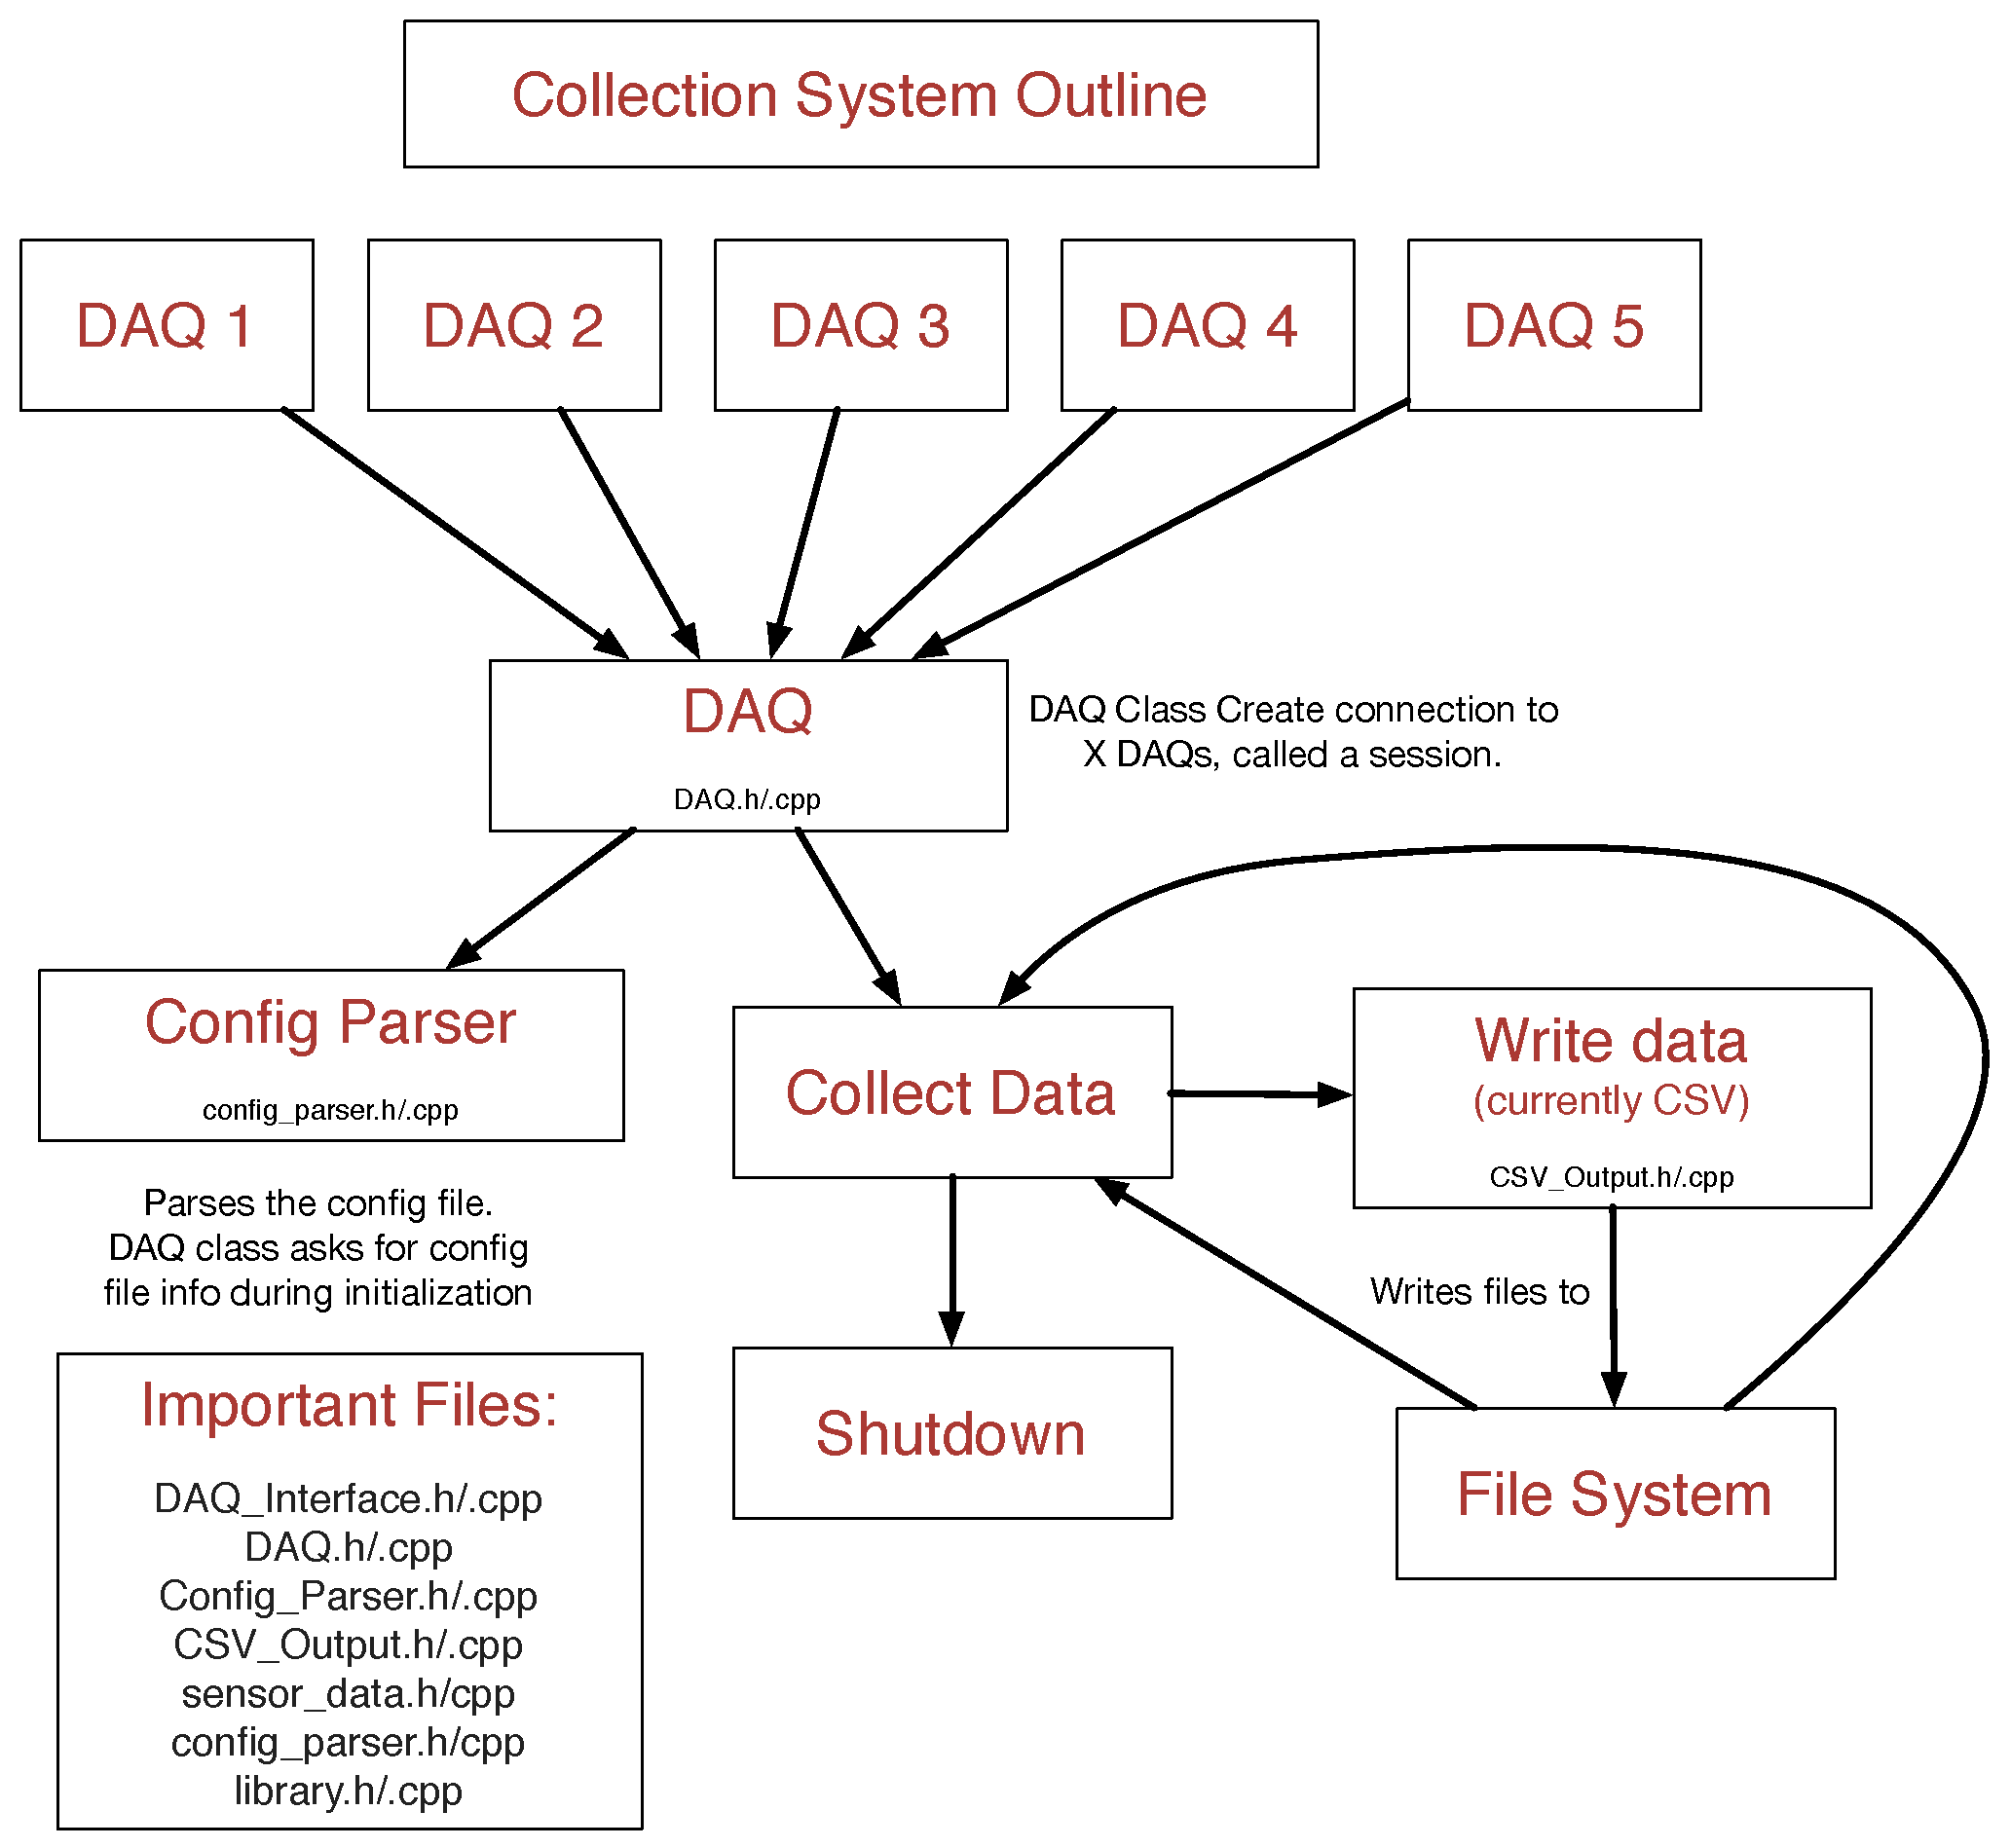
\includegraphics[width=5.5in]{figures/DAQ_collection_system_design.eps}
\caption{Collection system design.}
\label{fig:daq_collection_system_design}
\end{figure}

\section{Overview of Code Flow}
\label{sec:overview_of_code_flow}

In Figure \ref{fig:daq_collection_system_code_flow} is an outline of the flow of operation according to the code. 
This is more detailed than the overview of the system design in Section \ref{sec:overview_of_system_design}. 
Note that each file has an explanation in Section \ref{ch:documentation_for_each_class}.
Following the figure, the resource string from the command line (more details on the resource string in Section \ref{sec:data_pipeline}) is used to initialize the the session with the DAQ(s). 
The initialization function in DAQ.cpp (1) is called to set-up the connection (session) with the DAQ(s). 
This includes setting all the necessary parameters for the session. 
Here the configuration file (Section \ref{sec:config_file}) is parsed and user specified parameters are set. 
Then the collection cycle is started by the DAQ\_Interface object (2) in which the DAQ object's function continuousRawData() (3) is called. 
This function talks to the DAQ(s) and pulls records as they become available (4). 
Note that the settings within the code is set-up so the user does not need to worry about setting the Record Size (Section \ref{sec:parameters_and_data_structures}). 
The Record Size is set to the Sample Rate (Section \ref{sec:parameters_and_data_structures}) so that one record equals one second of data.  
After a certain number of records are collected (5) writeDaqDataToFile() is called and the CSV\_Output object writes the data to disk (6). 
Since a record equals one second of data, the number of records collected per file is specified in the configuration file. 
Then in (7), the buffer holding the data is flushed and the collection starts again for the next time slice (8). 
At any point during the collection phase, the user can press `e' (for end) to close the session and shutdown (9). 
During this process, any data that remains in the buffer is written to disk, i.e., a file containing a partial time slice is written to disk.


\begin{figure}
\centering
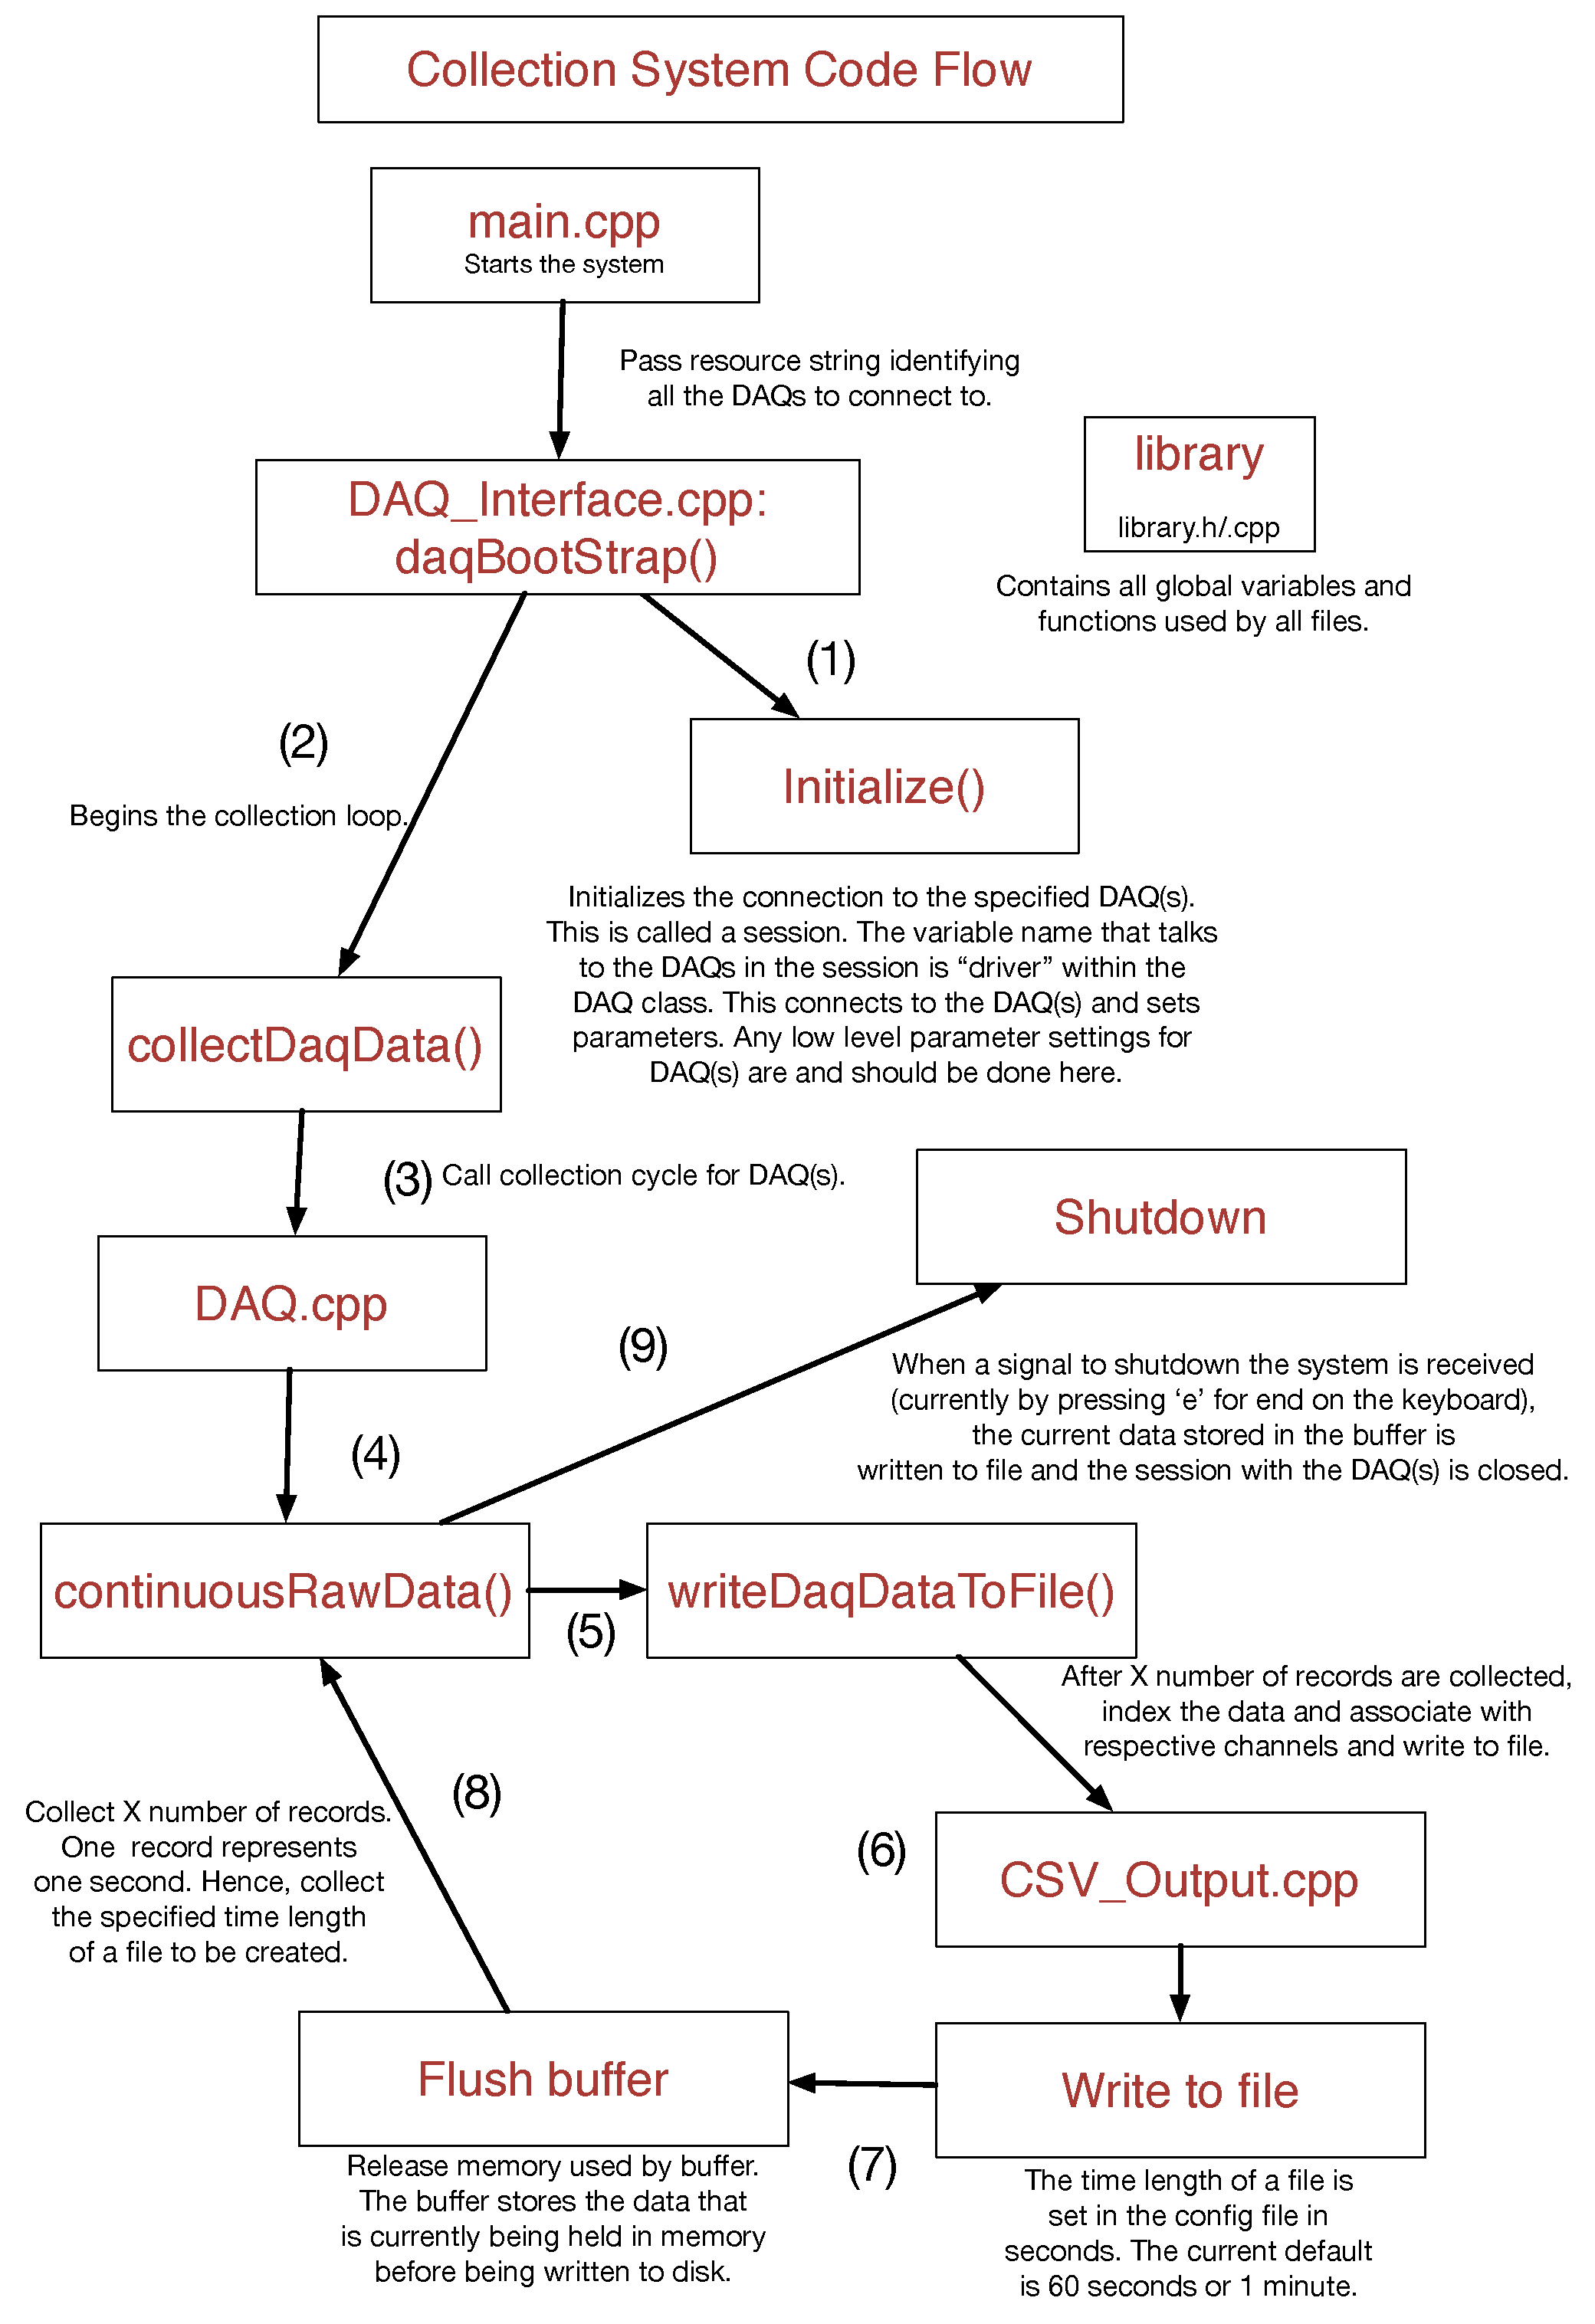
\includegraphics[width=5.5in]{figures/DAQ_collection_system_code_flow.eps}
\caption{Collection cycle overview: The continuousRawData() stores data to a buffer until a specified timeframe has passed for collection, i.e., the time length of a file. Once this is reached, steps (5) $\rightarrow$ (6) $\rightarrow$ (7) $\rightarrow$ (8) are executed. Here the data is written to file, the buffer is flushed, and then data is collected for the next timeframe.}
\label{fig:daq_collection_system_code_flow}
\end{figure}


\chapter{Documentation for each Class}
\label{ch:documentation_for_each_class}

\subsection{main.cpp}
This is the normal main of any C++ code base. 
It starts the whole system through creating the appropriate object(s) and then makes the function (of the appropriate object, currently the DAQ\_Interface class, but should be changed to the DAQ class) call that starts the entire collection cycle. 


\subsection{DAQ\_Interface.h/cpp}
This class was initially used to act as a controller for all the DAQs the collection system connects to, an interface to them. 
Each DAQ would have an instance of the DAQ class (next section) to handle interacting with the respective DAQs. 
Each instance would create a connection to a DAQ through what is called a \textit{session} historically named \textit{driver} in the code provided by VTI. 
However, after learning more about how to synchronize the DAQs, only one session is needed and hence, only one DAQ class instance. 
This resulted in the DAQ\_Interface acting as a controller for operating the one DAQ instance.
%class being unnecessary as it only adds another layer to the code flow that is not needed. 
%\textbf{As a result, the DAQ\_Interface class needs to be removed.}

\subsection{DAQ.h/cpp}
This class was initially meant to represent a connection (session - defined in previous section) to a single DAQ. 
After learning more about how to connect and synchronize to multiple DAQs, only one instance of this class was needed. 
Hence, one object of this class is used to control all the interactions with the DAQs. 
These are the following operations performed by this class:

\begin{itemize}
	\item \textbf{Initialize:} Establish a connection to DAQ(s) connected to the local network given a resource string defining the IP addresses or hostnames of each DAQ. Here all the desired parameters of the DAQ(s) are set such as the sample rate and system flags such as collecting only from DAQ channels with sensors. 
	\item \textbf{Collect Data:} As the DAQ(s) to provide a record of data from each. The data is returned in records which is defined in Section \ref{sec:parameters_and_data_structures}. Once a specified number of records is collected, the data is written to a specified medium, e.g., a CSV file.
	\item \textbf{Write to Medium:} This simply passes the information needed to the specified output medium for saving the data. After this is done, the currently held data is flushed for the next batch (memory released).
\end{itemize}


\subsection{Data\_Output.h/cpp}
This is a base class for performing inheritance in which multiple output methods can be defined, e.g., CSV or HDF5. 
Currently only CSV is defined, but using inheritance allows for flexibility to define others in the future. 

\subsection{Data\_Output\_Factory.h/Data\_Output\_Factory\_Implementation.h}
This is how different output types are created in C++. 
The factory creates a specified output object, e.g., a CSV object of the CSV\_Output class (next section). 
The implementation is written in a .h file as is historical practice. 

\subsection{CSV\_Output.h/cpp}
This class provides the method to write the DAQ data to a CSV file. 
A majority of this class is in the method that takes in the appropriate parameters from the DAQ class object so as to be written to file. 
This class contains the logic for indexing the DAQ data so as to organize the data by channel. 

\subsection{config\_parser.h/cpp}
This class parses the configuration file that defines specific user defined parameters. 
The format of this file is defined in Section \ref{sec:config_file}. 
The DAQ class uses this class to set respective parameters for the DAQ(s). 
Currently, the name and location of the configuration file is hard-coded to be called ``config\_file.txt'' located in the build directory. 

\subsection{library.h/cpp}
This contains all the shared functions and global variables. 
This allows multiple classes to use the same functions and variables for various tasks, e.g., a conversion function or a global flag. 

\subsection{sensor\_data.h/cpp}
This function acts as a wrapper for data from the DAQ(s). 
This data includes the SAFEARRAY containing the actual data and the BSTRs containing the timestamp information. 

\chapter{Hardware}
\label{ch:hardware}

\begin{itemize}
	\item \textbf{Hardware Inventory:}  \href{https://drive.google.com/open?id=1PWGKZkBGUQdU9gfNwpOJsPL04qn9HBuK3iqWUrPnyt4}{This spreadsheet} lists all the DAQs, cards, etc.
	\item \textbf{Map of Accelerometer Locations:} PDF map of where the accelerometers are located in Goodwin Hall: \href{https://drive.google.com/open?id=0B1KV5nIOprL6T1ZFdDRHZDlCNEU}{Accelerometer Locations}
		\item \textbf{DAQ User Manuals:}
		\begin{itemize}
			\item \href{https://drive.google.com/open?id=0B1KV5nIOprL6STYzc1VnY3JRdVE} {Manual for EMX 2500}
			\item See also the VTI Instruments product page for the \href{http://vtiinstruments.com/Products-Services/EMX-Series/EMX-2500.aspx}{EMX 2500 manual}. 
			\item \href{https://drive.google.com/open?id=0B1KV5nIOprL6STYzc1VnY3JRdVE}{Manual for EMX 4250, 4350, 4380} 
			\item See also the VTI Instruments product page for the \href{http://vtiinstruments.com/Products-Services/EMX-Series/EMX-4250.aspx} {EMX 4250, 4350, 4380.}
		\end{itemize}

\end{itemize}

\chapter{Software}
\label{ch:software}
This chapter details the software of the collection system. 


%\section{Instructions for Operating}
%\label{sec:instructions_for_operating}
%
%\todo{ADD: Running strictly using terminal}

\section{Data Pipeline}
\label{sec:data_pipeline}

Here we describe how the data gets to the collection system and its journey through the collection system until it is written to disk:

\begin{enumerate}
	\item A session is opened that connects to X number of DAQs - X is defined in the session connect call. E.g.,
	\begin{itemize}
		\item driver = new IVTEXDsaPtr(\_\_uuidof(VTEXDsa)); $\rightarrow$ create the object (named driver) that will talk to the DAQ
		\item driver$\rightarrow$Initialize(resource\_str, VARIANT\_FALSE, VARIANT\_TRUE, ""); $\rightarrow$ connects to the DAQs defined in the resource\_str (list of address strings), format is: ``TCPIP::IP\_\linebreak address\_1::INSTR$|$TCPIP::IP\_address\_2::INSTR$|$..." where ``$|$" is a vertical pipe.
		\item If a hostname is given to a DAQ, that can be used in the place of the address strings: "DAQ-4E.local$|$DAQ-1E.local$|$...". Note the ``.local" is needed to tell the system it is a local hostname. The actual host name does not have the ``.local". \textbf{The order of the hostnames is the order the data is given by the DAQs}. I.e., if the first hostname is DAQ-4E.local, then the first X number of channels will be from the DAQ with that hostname, where X is the number of channels on that DAQ. If the second DAQ is DAQ-1E.local, then the next Y channels will be from the DAQ with that hostname, where Y is the number of channels on that DAQ.
		\item This allows LAN synchronization in which the connected DAQs are time synced, i.e., all samples from all DAQs are synchronized in time. 	
		\item This is useful since when the data comes in, it is in the same format as if data from a single DAQ, hence, no changes needed in code after the few lines for synchronization.
	\end{itemize}
	\item During the initialization of the session with the DAQs, the configuration file is read in.
	\item Then collection of data is started. The data is read from the DAQ memory (memory stream call). Each record for each channel in all DAQs are pulled in parallel making for fast acquisition.
	\item After a specified number of records are pulled from the DAQs, those records are sent to be written to disk. 
	\begin{itemize}
		\item A file containing the sensor data (sensor readings and timestamps for all sensors) is created in for a specified time slice.
		\item E.g., Each file can represent data from a 1 minute time slice or 10 minutes. \textbf{The setting for this is in seconds.}

	\end{itemize}
\end{enumerate}

\section{Configuration File}
\label{sec:config_file}
A configuration file (config file) is provided to set certain parameters to specified values. 
This allows the user to specify relevant values without needing to set them in the code. 
The format consists of a header describing the different lines of the config file. 
These lines begin with a '\#' to signify to the parser to ignore them. 
For lines that contain parameter values, they are numbered with a value following. 
A semi-colon delimiter (';') is used between the numbered line and the value since it is an uncommon character. 
If a colon ':' or comma ',' are used, there may be parsing problems given some values may include them. 
An example of a config file is as follows:

\begin{description}
\itemsep-.5em 
	\item \#DAQ configuration set-up description
	\item \#All lines begin with a special identifier for a values
	\item \#	0; B $\rightarrow$ set clock frequency
	\item \#	1; C $\rightarrow$ set prescaler
	\item \#	2; D $\rightarrow$ set sample rate
	\item \#	3; E $\rightarrow$ length in seconds of each file produced
	\item \#	4; Move Path: set the path where collection files are stored locally. \textbf{NOTE:} need quotes around path and \textbackslash \textbackslash instead of \textbackslash.
	\item \#	5; Store all channel data: bool to specify to store all channel data, or just channels with sensors, value: 1 to store all, value 0: only with sensors
	\item \#	6; Display records to be collected on DAQ. This will show how many records are currently on the DAQ. This is good for monitoring if the records are being produced faster than can be collected and processed. This shows if the collection program can keep up with the DAQ.
	\item \#
	\item \#	DAQ $\rightarrow$ begin of configuration parameters for DAQ
	\item DAQ
	\item 0;204800
	\item 1;1
	\item 2;1600
	\item 3;60
	\item 4;``C:\textbackslash \textbackslash Users\textbackslash \textbackslash itsloaner\textbackslash \textbackslash Downloads\textbackslash \textbackslash SIL\_Collection\_Data"
	\item 5;0
	\item 6;1
	\item \#End of config file
\end{description}

%\todo{documentation on setting record size so user does not need to worry about it}

\section{Parameters and Data Structures}
\label{sec:parameters_and_data_structures}

Here are the definitions of the parameters used by the system. 
This includes what the values mean, how it is calculated, and what each is based on. 

\textbf{Clock Rate or Clock Frequency:}

\begin{itemize}
	\item This is either 204,800 or 131,072.
	\item This can be set in the code: driver$\rightarrow$Measurement$\rightarrow$Sampling$\rightarrow$ClockFrequency.
	\item Data Structure: integer
\end{itemize}

\textbf{Sample Rate:}

\begin{itemize}
	\item This is the number of samples taken per second.
	\item This can only be set to a 2 divisor of the Clock Rate.
	\begin{itemize}
		\item E.g., if the Clock Rate is 204,800, then the sample rates can be: 400, 800, 1600, 3200,..., 204,800.
	\end{itemize}
	\item The Sample Rate is calculated using the equation: \linebreak ClockFrequency\textbackslash Prescaler \/ $2^x$ where x is a number from 0 through 16.
	\item Data Structure: float
\end{itemize}

\textbf{Prescaler:}

\begin{itemize}
	\item Either set to 1 or 5. Default is 1.
	\item I do not touch this as it affects the calculations of the other parameters (see equation above).
	\item Data Structure: integer
\end{itemize}

\textbf{Record Size:}

\begin{itemize}
	\item The number of samples returned per record.
	\item A record is a unit used to store samples. The samples from the DAQs are returned in record form.
	\item E.g., if a record size is 10, then 1 record for 20 channels is 200 samples.
	\item \textbf{NOTE: This parameter is not set in the config file as it is just the way the DAQ driver handles the data. The record size is set automatically based on the defined sample rate. The record size is set to the sample rate so one record contains one second of data. Hence, a file time length can accurately be defined in increments of 1 second.}
	\item Data Structure: integer
\end{itemize}

\textbf{Record Size \/ Sample Rate:}

\begin{itemize}
	\item This gives the time slice of the samples in a record.
	\item E.g., for Sample Rate 1600Hz and Record Size 160, then $160 / 1600 = 0.1$ samples per second $\rightarrow$ returning samples every tenth of a second.
	\item This shows up as the samples in each record within a tenth of a second will have the same time stamp (e.g., 0.1). The next set of samples will have the time stamp 0.2 and so on.
\end{itemize}

\textbf{Sample Rate * Number of channels:}

\begin{itemize}
	\item This is the number of samples collected every second.
\end{itemize}

\textbf{Channel ID:}

\begin{itemize}
	\item This is the unique identifier for each channel.
	\item The channel ID is returned along with the sensor data.
	\item The format of the channel ID is:
	\begin{itemize}
		\item DAQ\#$<$no space$>$Card Slot \#$<$no space$>$!$<$no space$>$Channel \#
	\end{itemize}
	\item E.g., For DAQ 2, card slot 3, channel 6:
	\begin{itemize}
		\item 103!CH6
		\item DAQ\#$<$no space$>$Card Slot \#$<$no space$>$!$<$no space$>$Channel \#
		\item \textbf{NOTE: DAQ \# is in increments of 10, so DAQ 1 is $<$empty, no space or anything$>$, DAQ 2 is 10, DAQ 3 is 20, and so on.}
	\end{itemize}
	\item Data Structure: BSTR
\end{itemize}

\textbf{Timestamps:}

\begin{itemize}
	\item The timestamp is provided in 2 pieces: Seconds  (variable name: ts\_sec), and fractions of a second (variable name: ts\_frac).
	\item The seconds is the Unix epoch time, i.e., the number of seconds since January 1st 1970.
	\item The fractions of a second provide accuracy to the nanosecond.
	\item Data Structure: SAFEARRAYs for each. Both SAFEARRAYs are synced with each other as in index i for ts\_sec corresponds to index i in ts\_frac. Then both pieces together give the full timestamp which allows higher accuracy.
	\item Both variables are SAFEARRAYs that are the same size as the channels bstr. When requesting one record from a memory read, each sample in a record (record is X number of samples) for each channel has the same timestamp. Hence, everything in one record has the same timestamp.
	\item To provide an exact timestamp for each sample from the DAQ(s), the timestamp of the first record of a file is recorded along with the sample rate and the length of the file (in seconds). Then with this information, the timestamps for each sample can be calculated. 
	\item In other words, to get the exact time for each sample, one needs the time of the first sample ($t_0$) collected and the sample rate ($f_s$). Where the time step ($\Delta t$) is calculated:
	
	% Requires the booktabs if the memoir class is not being used
	\begin{table}[htbp]
	   \centering
	   %\topcaption{Table captions are better up top} % requires the topcapt package
	   \begin{tabular}{|c|} % Column formatting, @{} suppresses leading/trailing space
	      \hline
	%      \multicolumn{2}{c}{Item} \\
	%      \cmidrule(r){1-2} % Partial rule. (r) trims the line a little bit on the right; (l) & (lr) also possible
	%      Animal    & Description & Price (\$)\\
	 %     \midrule
	      $t_0$  \\
	      \hline
	      $t_0 + \Delta t$  \\
	      \hline
	      $t_0 + \Delta t * 2$  \\
	      \hline
	      ... \\
	      \hline
	      ... \\
	      \hline
	      $t_0 + \Delta t * n$  \\
	      \hline
	   \end{tabular}
	   \caption{Example calculation of the time of each sample in a file. Note: n is the last line in the file.}
	   \label{tab:booktabs}
	\end{table}
\end{itemize}

\section{Setting up Development Environment}
\label{sec:setting_up_development_environment}

Here is the list of software and steps for installing the needed software to develop with the DAQs.

\begin{itemize}
	\item A tool to identify LXI devices that are attached to the network must be installed: \href{http://lxistandard.org/Resources/LXIDiscoveryTool.aspx}{LXI Discovery Tool}. This is needed since it forces you to install Apple Bonjour print services which is required to connect to the DAQs via their hostname (and not IP).
	\item Have the latest version of Microsoft Visual Studio. This is used to provide the computer with a compiler. 
	\item In order to interface with the DAQ you have to install the following (in this order, \textbf{VERY IMPORTANT!}):
	\begin{enumerate}
		\item \href{http://www.microsoft.com/en-us/download/details.aspx?id=8279}{Windows SDK (windows 7) and .NET Framework 4} 
		\item \href{http://www.ivifoundation.org/shared_components/}{IVI Shared Components}
		\item \href{http://www.vtiinstruments.com/Support-and-Resources/Documents-and-downloads.aspx?searchtext=IVI+DSA&searchmode=anyword&searchfilter=0}{VTI's EMX Driver}
	\end{enumerate}
	\item In order to interface with the thermal coupler hardware (EM-1048A):
	\begin{enumerate}
		\item The \href{http://www.vtiinstruments.com/files/DRIVERS/DRIVER,64BIT,SOFT\%20FRONT\%20PANEL,PLUG\%20AND\%20PLAY,EX10xxA_R1P4P0.zip}{PNP driver} assuming 64 bit WindowsOS.
		\item The \href{http://www.vtiinstruments.com/files/IVI/DRIVER,IVI,32B_64B_EX10XXA_R1P4P0.zip}{IVI driver}.
		\item Password for access to IVI driver to make changes through web interface: ex1048
	\end{enumerate}
	\item For Qt development environment (includes Qt Creator) - available from \burl{https://www.qt.io/download-open-source/}
\end{itemize}

\section{Software Versioning}
\label{sec:software_versioning}

Here is described a simple introduction to software versioning. 
Versioning is used to keep a history of changes and allow a safety net for development and protect against breaking a code base. 
In Figure \ref{fig:version_control_flow}, we see a simple flow of how versioning (or version control) works. 
One starts with a \emph{master} version of the code. 
This is the stable version that is meant to see the light of day.
This version is never touched unless what is being added is known to be stable. 
Because of this, a \emph{working development} branch is created for development. 
When a new feature wants to be tested, a new branch is created (\emph{cool feature 1}). 
The code in this branch is developed and tested until the operation is satisfactory. 
Then that code is merged back into the \emph{working development}. 
Now \emph{working development} has the new cool feature 1. 
This is continued until a stable version of \emph{working development} is reached and is ready to be merged back into \emph{master}. 
After which, the cycle continues for the life of the code. 


\begin{figure}
\centering
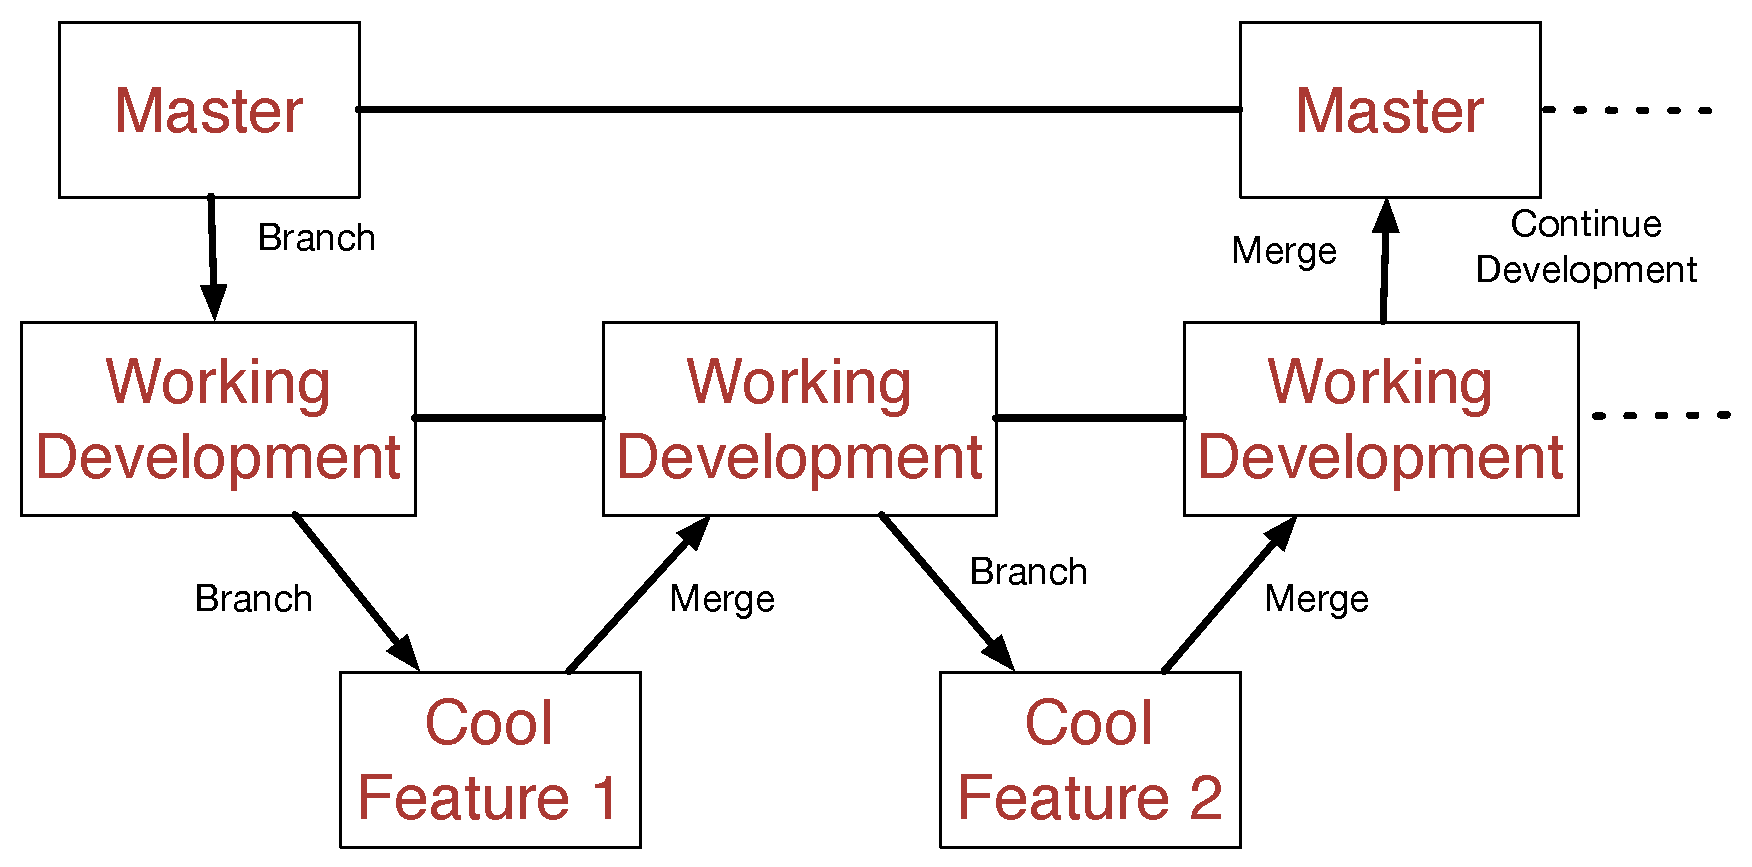
\includegraphics[width=5.5in]{figures/Version_Control_Flow.eps}
\caption{Example of how versioning works. One starts with a \emph{master} version of the code. Then a \emph{working development} branch is created for development. When a new feature wants to be tested, a new branch is created (\emph{cool feature 1}). When the operation of the feature is satisfactory, that code is merged back into the \emph{working development}. When the \emph{working development} is stable, it is merged back into \emph{master}. }
\label{fig:version_control_flow}
\end{figure}

\section{Code Base and Github}
\label{sec:code_base}

The C++ code base is stored in a GitHub repository at 
\begin{itemize}
	\item \burl{https://github.com/VTUL/VT-SIL-Collection-System}
\end{itemize}
To gain access to this repository, you can fork or clone it. 
To clone (i.e., download project and entire version history) use the following command from the github power shell:
\begin{itemize}
	\item git clone \burl{https://github.com/VTUL/VT-SIL-Collection-System}
\end{itemize}
It will download the code base into the folder ``smart-infrastructure-laboratory" in the current directory. 

Assuming, the user already understands versioning of software, the following commands are what is needed for development:
\begin{itemize}
	\item git branch 
	\item git branch [branch-name]
	\item git status
	\item git add
	\item git rm
	\item git commit -m ``useful message"
	\item git push origin [current\_branch\_name]
\end{itemize}
\textbf{Please refer to Appendix \ref{appendix_github_reference_sheet} for more details and explanations on git commands.}

When committing changes and saving to github, perform the following commands:
\begin{itemize}
	\item git status $\rightarrow$ See what files have been changed.
	\item git add $\rightarrow$ Add any files that were changed (one `git add' per file)
	\item git commit -m ``useful message" $\rightarrow$ Commit changes to the local repository on the computer. The message is for describing what the changes are.
	\item git push origin [current branch-name] $\rightarrow$ Pushes the changes to github.
\end{itemize}
To see what the current branch-name is, use the command: 
\begin{itemize}
	\item git branch
\end{itemize}	
To change branches, use the command: 
\begin{itemize}
	\item git checkout $<$branch\_name$>$
\end{itemize}

In order to download and allow synching with a specific branch on github that you do not currently have on your machine, use the following command:
\begin{itemize}
	\item git checkout -b some\_branch origin/branch\_name
\end{itemize}
For example, to to get the branch \textit{cool\_branch}, the command is: 
\begin{itemize}
	\item git checkout -b cool\_branch origin/cool\_branch
\end{itemize}
\textbf{NOTE: Do not use spaces in your branch names!!}

When someone else makes changes in a branch and uploads it to github, in order for you to get those changes on your local machine, all you need to do is use the following command when you are in the branch that has changes:
\begin{itemize}
	\item git pull
\end{itemize}



\section{Running the System}
\label{sec:running_the_system}
Here is described how to run the system for collection of data. 
The system can be run from a console with a simple command. 
To do this, what needs to be known is:
\begin{itemize}
	\item Location of executable.
	\item Location of configuration file.
	\item The DAQ network IDs that one wants to connect to.
\end{itemize}

In the current setting for development and since github is being used, the location of the source code will be:
\begin{itemize}
	\item C:\textbackslash Users\textbackslash $<$user name$>$\textbackslash Documents\textbackslash Github \textbackslash VT\_SIL\_DAQ\_Interface
\end{itemize}
Where $<$user name$>$ is the account name currently logged into on the computer.


The locations of the debug and release versions of the executable will be:
\begin{itemize}
	\item Debug: C:\textbackslash Users\textbackslash $<$user name$>$\textbackslash Documents\textbackslash Github \textbackslash VT\_SIL\_DAQ\_Interface\textbackslash build\textbackslash debug
		\item Release C:\textbackslash Users\textbackslash $<$user name$>$\textbackslash Documents\textbackslash Github \textbackslash VT\_SIL\_DAQ\_Interface\textbackslash build\textbackslash release
\end{itemize}

If running the system from an IDE such as Qt Creator, the config file (named daq\_config.txt) must be in the following location:
\begin{itemize}
	\item Debug: C:\textbackslash Users\textbackslash $<$user name$>$\textbackslash Documents\textbackslash Github \textbackslash VT\_SIL\_DAQ\_Interface\textbackslash build
\end{itemize}

If running the system from the command line, the config file (named daq\_config.txt) must be in the following location for debug and release, respectively:
\begin{itemize}
	\item Debug: C:\textbackslash Users\textbackslash $<$user name$>$\textbackslash Documents\textbackslash Github \textbackslash VT\_SIL\_DAQ\_Interface\textbackslash build\textbackslash debug\textbackslash
		\item Release: C:\textbackslash Users\textbackslash $<$user name$>$\textbackslash Documents\textbackslash Github \textbackslash VT\_SIL\_DAQ\_Interface\textbackslash build\textbackslash release\textbackslash
\end{itemize}

To run \textbf{using Qt Creator}, double-click the project .pro file located in:
\begin{itemize}
	\item C:\textbackslash Users\textbackslash $<$user name$>$\textbackslash Documents\textbackslash Github \textbackslash VT\_SIL\_DAQ\_Interface\textbackslash DAQ\_Interface.pro
\end{itemize}

Or use the alias on the desktop (if available). 
To enter which DAQ(s) to connect to, go to the Project settings on the left-hand side, then to Run (top of settings screen). 
There is a line for arguments. 
Enter the DAQ resource string as described in Section \ref{sec:data_pipeline}. 
While your cursor is in the arguments box, hit `enter' then save (control+s) to have the resource string you just entered to stick. 
I do not know why, but this must be done. 

To run from \textbf{command line}, open a power shell using Github, an alias should be on the desktop. %ConEmu (installed and alias on desktop). 
%If ConEmu is not installed, it can be downloaded from: \burl{http://www.fosshub.com/ConEmu.html}. 
The power shell is provided when installing Github for Windows. 
%In ConEmu, the current console shown can be set to a power shell through using the drop-down menu for that console tab. 
%The power shell is very useful as it operates like a Linus/Unix/Mac terminal. 
Using the power shell, navigate to either the debug or release folder described above. 
Then the command to run is:
\begin{itemize}
	\item DAQ\_Interface.exe ``$<$resource string$>$" $<$then hit enter$>$
	\item Where $<$resource string$>$ is as described in Section \ref{sec:data_pipeline}. 
	\item An example: DAQ\_Interface.exe ``DAQ-4E.local"$\rightarrow$ to start the system connecting to DAQ-4E
	\item An example: DAQ\_Interface.exe ``DAQ-4E.local$|$DAQ-1E"$\rightarrow$ to start the system connecting to DAQ-4E and DAQ-1E (in that order).
\end{itemize}

\textbf{To stop the system type 'e' for `end' while the power shell window is in focus.}

\section{Technical Details}
\label{sec:technical_details}
Described here are details about using the IVI driver for the DAQs in terms of working with their data structures. 
Think of this is as a ``lessons learned" section for technical details.
\begin{itemize}
	\item The data format used by the DAQs for storing sensor and other data: For each record returned by the DAQ, the sensor data is one long array of values with the first X values belonging to channel 1, the next X to channel 2 and so forth, where X is the record size, i.e. how many sensor points per record.
	\item All this data is stored in a SAFEARRAY, a data structure optimized for passing to COM objects (e.g., storing in shared memory so another program can use it, just like a copy-paste clipboard). To access the sensor data, the example code for the DAQ driver shows how to iterate through the sensor data one value at a time.
	\item To speed up the system, the SAFEARRAY for each record is stored to avoid iterating through the data more than once. Then when it came time to write to disk, iterate through the SAFEARRAY by "jumping" around to pull out all the data for channel 1 in all the records, then for channel 2 and so forth so. This would put all the values for each channel together and lead to linear time access to the SAFEARRAY as each element is accessed only once.
	\item When accessing multiple elements from a SAFEARRAY, it is best to use SafeArrayAccessData() before accessing and SafeArrayUnaccessData() when done. An example can be seen here: \burl{https://msdn.microsoft.com/en-us/library/ms221620.aspx}. Also a code snippet from the system is below: 
\begin{lstlisting}
 double *currentSensorDataDouble;
HRESULT hr;
// Get a pointer to the elements of the array.
hr = ::SafeArrayAccessData(currentSensorData->getData(), (void**)&?currentSensorDataDouble?);?


if (FAILED(hr)){
    cout<<"Error getting access to SAFEARRAY of sensor data. Aborting..."<<endl;
    return;
}

double dd = 0.0;
for (int i = 0; i < currentSensorData->getData()->rgsabound->cElements; i++)
{
    dd = (double)currentSensorDataDouble[i];
    outputStdStr.append(std::to_string(dd));
}
\end{lstlisting}

\item Accessing the data this way, allowed writing the data to a CSV file with each column representing the sensor data from one channel.

\end{itemize}

\section{Challenges and Solutions}
\label{sec:challenges_and_solutions}
Here is described a number of challenges faced along the way. 
Solutions to some of these challenges are provided, but not all currently have solutions. 

\subsection{DAQ Buffer Filling Up}
This by far has been the biggest challenged faced to date. 
This entailed writing sensor data to disk fast enough to keep up with the data streaming in from the DAQ(s). 
On can find out if the collection system is keeping up by pinging the DAQs for how many records are currently ready. 
If that number is increasing, then the onboard DAQ memory will slowly fill up and sensor data will eventually be lost. 

Methods performed to streamline speed:
\begin{itemize}
	\item Not using Qt in the collection system. Using the QString data structure for storing data before writing to disk ended up being slow since the QString needed to be converted to a standard C++ string to be written out. This conversion was very slow with so much data ( ~5 times slower).
	\item Changing to using standard C++ strings speed up the collection system considerably. 
	\item Simplifying the file I/O to one write per file created. This is done by collecting all the sensor data for Y records, then writing to disk once. The sensor data is stored in a C++ standard string before being written to disk. The string is used to provide proper formatting for the output file, e.g., CSV file with header(s). Once written, the memory (RAM) used by this string is reclaimed by the computer.
	\item One thing discovered is any method for writing a string to file was about the same speed. This includes using the C++ output operator $<<$ and C style writing to disk (outStream(buffer,size) where size is the length of the buffer).
\end{itemize}

It was discovered that the source of the slowdown is converting the sensor value (in the form of a double) to a string that can be written to disk. 
It is this conversion from a floating point number to a string that is considerably slow. 
Currently, there appears to not be any conversion that is faster. 
In the future using different output file types, e.g., HDF5 or binary, may increase the speed. 
However, when the system is run in `release mode' instead of `debug mode', the conversion is $\sim15$ times faster. 
Due to the speed provided by release mode, the entire collection system can run and keep up with the data from the DAQ(s). 
%This slowdown is noticed since the collection system is dealing with hundreds of thousands of sample points. 

\subsection{Slow-down in Windows 8.1}
\label{sec:slow_down_in_windows_8_1}

There appears to be a known problem in Windows 8.1 where code compiled using Microsoft Visual Studio compiler VS2013 is $\sim50$\% slower than in Windows 7. 
I observed this when running the code on the SIL desktop. 
On the Windows 7 laptop used for development, the system was faster despite the fact that the desktop is significantly more powerful. 
If possible, it is recommended to use Windows 7 for the new server. 
However, the server should have Windows Server (2008 or 2012) at some point. 
But before that, testing running the system on Windows Server would need to be done on a separate computer to verify operability. 

\section{Data Storage}
\label{sec:data_storage}

The data is sent to the Advanced Research Computing (ARC) group at Virginia Tech for storage: \burl{http://www.arc.vt.edu/}. 
There is a script that performs sending the data to ARC.

\todo{what is this script??} 

\chapter{Currently Known Problems}
\label{ch:currently_known_problems}
Here is describe the currently know problems with the system. 
This can be seen as a `Todo' list of important problems to be addressed for future development. 

\begin{enumerate}
	\item \textbf{Large memory leak:} Somewhere is a large memory leak. A potential source is the BSTRs not used that are returned from the Memory Read. These may need to be stored in the Sensor\_Data class like the sensor data and time stamps, then release in the same manner. When trying to release these BSTRs in the collection loop, it works with 1 DAQ but not with 5 for some reason. 
\end{enumerate}

%Appendices
\appendix

\chapter{Github Reference Sheet}
\label{appendix_github_reference_sheet}

\begin{figure}
\centering
\includegraphics[width=7.5in]{figures/Github_reference_sheet_pg_1.eps}

\caption{Github reference sheet (page 1).}

\label{fig:github_reference_sheet_page_2}
\end{figure}

\begin{figure}
\centering
\includegraphics[width=7.5in]{figures/Github_reference_sheet_pg_2.eps}

\caption{Github reference sheet (page 2).}

\label{fig:github_reference_sheet_page_2}
\end{figure}


\end{document}


















